% Options for packages loaded elsewhere
\PassOptionsToPackage{unicode}{hyperref}
\PassOptionsToPackage{hyphens}{url}
%
\documentclass[
  letterpaper,
  ignorenonframetext,
  aspectratio=43,
  handout,
  12pt]{beamer}
\usepackage{pgfpages}
\setbeamertemplate{caption}[numbered]
\setbeamertemplate{caption label separator}{: }
\setbeamercolor{caption name}{fg=normal text.fg}
\beamertemplatenavigationsymbolsempty
% Prevent slide breaks in the middle of a paragraph
\widowpenalties 1 10000
\raggedbottom
\setbeamertemplate{part page}{
  \centering
  \begin{beamercolorbox}[sep=16pt,center]{part title}
    \usebeamerfont{part title}\insertpart\par
  \end{beamercolorbox}
}
\setbeamertemplate{section page}{
  \centering
  \begin{beamercolorbox}[sep=12pt,center]{part title}
    \usebeamerfont{section title}\insertsection\par
  \end{beamercolorbox}
}
\setbeamertemplate{subsection page}{
  \centering
  \begin{beamercolorbox}[sep=8pt,center]{part title}
    \usebeamerfont{subsection title}\insertsubsection\par
  \end{beamercolorbox}
}
\AtBeginPart{
  \frame{\partpage}
}
\AtBeginSection{
  \ifbibliography
  \else
    \frame{\sectionpage}
  \fi
}
\AtBeginSubsection{
  \frame{\subsectionpage}
}
\usepackage{amsmath,amssymb}
\usepackage{lmodern}
\usepackage{ifxetex,ifluatex}
\ifnum 0\ifxetex 1\fi\ifluatex 1\fi=0 % if pdftex
  \usepackage[T1]{fontenc}
  \usepackage[utf8]{inputenc}
  \usepackage{textcomp} % provide euro and other symbols
\else % if luatex or xetex
  \usepackage{unicode-math}
  \defaultfontfeatures{Scale=MatchLowercase}
  \defaultfontfeatures[\rmfamily]{Ligatures=TeX,Scale=1}
\fi
\usetheme[]{metropolis}
% Use upquote if available, for straight quotes in verbatim environments
\IfFileExists{upquote.sty}{\usepackage{upquote}}{}
\IfFileExists{microtype.sty}{% use microtype if available
  \usepackage[]{microtype}
  \UseMicrotypeSet[protrusion]{basicmath} % disable protrusion for tt fonts
}{}
\makeatletter
\@ifundefined{KOMAClassName}{% if non-KOMA class
  \IfFileExists{parskip.sty}{%
    \usepackage{parskip}
  }{% else
    \setlength{\parindent}{0pt}
    \setlength{\parskip}{6pt plus 2pt minus 1pt}}
}{% if KOMA class
  \KOMAoptions{parskip=half}}
\makeatother
\usepackage{xcolor}
\IfFileExists{xurl.sty}{\usepackage{xurl}}{} % add URL line breaks if available
\IfFileExists{bookmark.sty}{\usepackage{bookmark}}{\usepackage{hyperref}}
\hypersetup{
  hidelinks,
  pdfcreator={LaTeX via pandoc}}
\urlstyle{same} % disable monospaced font for URLs
\newif\ifbibliography
\usepackage{graphicx}
\makeatletter
\def\maxwidth{\ifdim\Gin@nat@width>\linewidth\linewidth\else\Gin@nat@width\fi}
\def\maxheight{\ifdim\Gin@nat@height>\textheight\textheight\else\Gin@nat@height\fi}
\makeatother
% Scale images if necessary, so that they will not overflow the page
% margins by default, and it is still possible to overwrite the defaults
% using explicit options in \includegraphics[width, height, ...]{}
\setkeys{Gin}{width=\maxwidth,height=\maxheight,keepaspectratio}
% Set default figure placement to htbp
\makeatletter
\def\fps@figure{htbp}
\makeatother
\setlength{\emergencystretch}{3em} % prevent overfull lines
\providecommand{\tightlist}{%
  \setlength{\itemsep}{0pt}\setlength{\parskip}{0pt}}
\setcounter{secnumdepth}{-\maxdimen} % remove section numbering
\usepackage{pgfpages}
\pgfpagesuselayout{2 on 1}
\providecommand{\tightlist}{%
\setlength{\itemsep}{0pt}\setlength{\parskip}{0pt}}
\makeatletter
\makeatother
\let\Oldincludegraphics\includegraphics
\renewcommand{\includegraphics}[2][]{\Oldincludegraphics[width=\textwidth,height=0.7\textheight,keepaspectratio]{#2}}
\ifluatex
  \usepackage{selnolig}  % disable illegal ligatures
\fi

\author{}
\date{}

\begin{document}

\begin{frame}
Lecture 2 - Tensor review, Anisotropic Elasticity

Dr.~Nicholas Smith

Wichita State University, Department of Aerospace Engineering

February 4, 2021
\end{frame}

\begin{frame}{schedule}
\protect\hypertarget{schedule}{}
\begin{itemize}
\tightlist
\item
  Feb 4 - Tensor review, Anisotropic Elasticity
\item
  Feb 9 - Coordinate Transformation
\item
  Feb 11 - 1D Micromechanics (HW1 Due)
\item
  Feb 16 - Orientation Averaging
\end{itemize}
\end{frame}

\begin{frame}{outline}
\protect\hypertarget{outline}{}
\begin{itemize}
\tightlist
\item
  index notation
\item
  anisotropic elasticity
\end{itemize}
\end{frame}

\hypertarget{index-notation}{%
\section{index notation}\label{index-notation}}

\begin{frame}{index notation}
\protect\hypertarget{index-notation-1}{}
\begin{itemize}
\tightlist
\item
  Consider the following
\item
  \emph{s} = \emph{a}1\emph{x}1 + \emph{a}2\emph{x}2 + \ldots{} +
  \emph{a}\emph{n}\emph{x}\emph{n}
\item
  Which we could also write as
\end{itemize}

\[s = \sum_{i=1}^{n}a_ix_i\]

\begin{itemize}
\tightlist
\item
  Using index notation, and Einstein's summation convention, we can also
  write this as \emph{s} = \emph{a}\emph{i}\emph{x}\emph{i}
\end{itemize}
\end{frame}

\begin{frame}{dummy index}
\protect\hypertarget{dummy-index}{}
\begin{itemize}
\tightlist
\item
  In index notation, a repeated index implies summation
\item
  This index is also referred to as a dummy index
\item
  It is called a ``dummy index'' because the expression would have the
  same meaning with any index in its place
\item
  i.e.~\emph{i}, \emph{j}, \emph{k}, etc. would all have the same
  meaning when repeated
\end{itemize}
\end{frame}

\begin{frame}{dummy index}
\protect\hypertarget{dummy-index-1}{}
\begin{itemize}
\tightlist
\item
  Note, no index may be repeated more than once, thus the expression
\end{itemize}

\[s = \sum_{i=1}^{n}a_ib_ix_i\]

could not be directly written in index notation
\end{frame}

\begin{frame}{free index}
\protect\hypertarget{free-index}{}
\begin{itemize}
\tightlist
\item
  Any index which is not repeated in an index notation expression is
  referred to as a free index
\item
  The number of free indexes in an expression indicate the tensor order
  of that expression
\item
  No free indexes = scalar expression (0-order tensor)
\item
  One free index = vector expression (1st-order tensor)
\item
  Two free indexes = matrix expression (2nd-order tensor)
\end{itemize}
\end{frame}

\begin{frame}{index notation}
\protect\hypertarget{index-notation-2}{}
\begin{columns}[T]
\begin{column}{0.5\textwidth}
\begin{itemize}
\tightlist
\item
  Free index is not repeated (on any term)
\item
  Free index takes all values (1,2,3)
\item
  e.g.~\(u_i = \langle u_1, u_2, u_3 \rangle\)
\item
  Free indexes must match across terms in an expression or equation
\end{itemize}
\end{column}

\begin{column}{0.5\textwidth}
Dummy index is repeated on at least one term Dummy index indicates
summation over all values
e.g.~\(\sigma_{ii} = \sigma_{11} + \sigma_{22} + \sigma_{33}\) Index can
not be used more than twice in the same term (\(A_{ij}B_{jk}C_{kl}\) is
good, \(A_{ij}B_{ij}C_{ij}\) is not)
\end{column}
\end{columns}
\end{frame}

\begin{frame}{dummy index}
\protect\hypertarget{dummy-index-2}{}
\begin{itemize}
\tightlist
\item
  The dummy index can be triggered by any repeated index in a
  \emph{term}.
\item
  Summation or not?

  \begin{itemize}
  \tightlist
  \item
    \(a_i + b_{ij}c_j\)
  \item
    \(a_{ij}b_{ij}\)
  \item
    \(a_{ij} + b_{ij}c_j\)
  \end{itemize}
\end{itemize}
\end{frame}

\begin{frame}{matrix multiplication}
\protect\hypertarget{matrix-multiplication}{}
\begin{itemize}
\tightlist
\item
  How can we write matrix multiplication in index notation?
\end{itemize}

\[\begin{bmatrix}
    a_{11} & a_{12} \\
    a_{21} & a_{22}
  \end{bmatrix}
  \begin{bmatrix}
    b_{11} & b_{12} \\
    b_{21} & b_{22}
  \end{bmatrix} =
  \begin{bmatrix}
    c_{11} & c_{12} \\
    c_{21} & c_{22}
  \end{bmatrix}\]
\end{frame}

\hypertarget{special-symbols}{%
\section{special symbols}\label{special-symbols}}

\begin{frame}{kronecker delta}
\protect\hypertarget{kronecker-delta}{}
\begin{itemize}
\tightlist
\item
  For convenience we define two symbols in index notation
\item
  \emph{Kronecker delta} is a general tensor form of the Identity Matrix
\end{itemize}

\[\delta_{ij} = \left\{
\begin{array}{ll}
  1& \text{if $i=j$}\\
  0& \text{otherwise}
\end{array}
\right. = \begin{bmatrix}
  1 & 0 & 0\\
  0 & 1 & 0 \\
  0 & 0 & 1
\end{bmatrix}\]

\begin{itemize}
\tightlist
\item
  Is also used for higher order tensors
\end{itemize}
\end{frame}

\begin{frame}{kronecker delta}
\protect\hypertarget{kronecker-delta-1}{}
\begin{itemize}
\tightlist
\item
  \(\delta_{ij} = \delta_{ji}\)
\item
  \(\delta_{ii} = 3\)
\item
  \(\delta_{ij} a_j = a_{i}\)
\item
  \(\delta _{ij} b_{ij} = b_{ii}\)
\end{itemize}
\end{frame}

\begin{frame}{alternating symbol}
\protect\hypertarget{alternating-symbol}{}
\begin{itemize}
\tightlist
\item
  \emph{alternating symbol} or \emph{permutation symbol}
\end{itemize}

\[\epsilon_{ijk} = \left\{
\begin{array}{rl}
  1 & \text{if $ijk$ is an even permutation of 1,2,3}\\
  -1 & \text{if $ijk$ is an odd permutation of 1,2,3}\\
  0 & \text{otherwise}
\end{array}
\right.\]
\end{frame}

\begin{frame}{alternating symbol}
\protect\hypertarget{alternating-symbol-1}{}
\begin{itemize}
\tightlist
\item
  This symbol is not used as frequently as the \emph{Kronecker delta}
\item
  For our uses in this course, it is enough to know that 123, 231, and
  312 are even permutations
\item
  321, 132, 213 are odd permutations
\item
  all other indexes are zero
\item
  \(\epsilon_{ijk} \epsilon_{imn} = \delta_{jm}\delta_{kn} - \delta_{jn}\delta{mk}\)
\end{itemize}
\end{frame}

\hypertarget{tensor-algebra}{%
\section{tensor algebra}\label{tensor-algebra}}

\begin{frame}{substitution}
\protect\hypertarget{substitution}{}
\begin{itemize}
\tightlist
\item
  When solving tensor equations, we often need to manipulate expressions
\item
  We need to make sure the correct indexes are used when substituting,
  for example
\end{itemize}

\[a_i = U_{im}{b_m} \label{eq:first} \tag{1}\]

\[b_i = V_{im}{c_m} \label{eq:second} \tag{2}\]

\begin{itemize}
\tightlist
\item
  To substitute (2) into (1), we first need to change indexes
\end{itemize}
\end{frame}

\begin{frame}{substitution}
\protect\hypertarget{substitution-1}{}
\begin{itemize}
\tightlist
\item
  We need to change the free index, \emph{i}, to \emph{m} in (2)
\item
  Since \emph{m} is already used as the dummy index, we need to change
  that too
\end{itemize}

\[b_m = V_{mj}{c_j} \label{eq:third} \tag{3}\]

\begin{itemize}
\tightlist
\item
  We can now make the substitution
\end{itemize}

\[a_i = U_{im}V_{mj}{c_j} \label{eq:fourth} \tag{4}\]
\end{frame}

\begin{frame}{multiplication}
\protect\hypertarget{multiplication}{}
\begin{itemize}
\tightlist
\item
  We need to be careful with indexes when multiplying expressions
\item
  \(p = a_m b_m\) and \(q = c_m d_m\)
\item
  We can express, \emph{pq}, but remember the dummy index cannot be
  repeated more than once
\item
  \(pq \ne a_m b_m c_m d_m\)\\
\item
  Instead we must change the dummy index in one of the expressions first
\item
  \(pq = a_m b_m c_n d_n\)
\end{itemize}
\end{frame}

\begin{frame}{factoring}
\protect\hypertarget{factoring}{}
\begin{itemize}
\tightlist
\item
  In the following expression, we would like to factor out \emph{n}, but
  it has different indexes
\item
  \(\sigma_{ij}n_j - \lambda n_i = 0\)
\item
  Recall \(\delta_{ij}a_j = a_i\) we can rewrite
  \(n_i = \delta_{ij}{nj}\)
\item
  \(\sigma_{ij}n_j - \lambda \delta_{ij}{nj} = 0\)
\item
  \((\sigma_{ij} - \lambda \delta_{ij}){nj} = 0\)
\end{itemize}
\end{frame}

\begin{frame}{contraction}
\protect\hypertarget{contraction}{}
\begin{itemize}
\tightlist
\item
  \(\sigma_{ii}\) is the contraction of \(\sigma_{ij}\)
\item
  This can often be a useful tool in solving tensor equations
\item
  \(\sigma_{ij} = \lambda \Delta \delta_{ij} + 2\mu E_{ij}\)
\item
  \(\sigma_{ii} = 3\lambda \Delta + 2\mu E_{ii}\)
\end{itemize}
\end{frame}

\hypertarget{tensor-calculus}{%
\section{tensor calculus}\label{tensor-calculus}}

\begin{frame}{partial derivative}
\protect\hypertarget{partial-derivative}{}
\begin{itemize}
\tightlist
\item
  We indicate (partial) derivatives using a comma
\item
  In three dimensions, we take the partial derivative with respect to
  each variable (\emph{x}, \emph{y}, \emph{z} or \(x_1\), \(x_2\), and
  \(x_3\))
\item
  For example a scalar property, such as density, can have a different
  value at any point in space
\item
  \(\rho = \rho(x_1, x_2, x_3)\)
\item
  \(\rho_{,i} = \frac{\partial}{\partial x_i} \rho = \left \langle \frac{\partial \rho }{\partial x_1}, \frac{\partial \rho }{\partial x_2}, \frac{\partial \rho }{\partial x_3} \right\rangle\)
\end{itemize}
\end{frame}

\begin{frame}{partial derivative}
\protect\hypertarget{partial-derivative-1}{}
\begin{itemize}
\tightlist
\item
  Similarly, if we take the partial derivative of a vector, it produces
  a matrix
\end{itemize}

\[u_{i,j} = \frac{\partial}{\partial x_j} u_i = \begin{bmatrix}
  \frac{\partial u_1}{\partial x_1} & \frac{\partial u_1}{\partial x_2} & \frac{\partial u_1}{\partial x_3}\\
  \frac{\partial u_2}{\partial x_1} & \frac{\partial u_2}{\partial x_2} & \frac{\partial u_2}{\partial x_3}\\
  \frac{\partial u_3}{\partial x_1} & \frac{\partial u_3}{\partial x_2} & \frac{\partial u_3}{\partial x_3}
\end{bmatrix}\]
\end{frame}

\hypertarget{dyadic-notation}{%
\section{dyadic notation}\label{dyadic-notation}}

\begin{frame}{dyadic notation}
\protect\hypertarget{dyadic-notation-1}{}
\begin{itemize}
\tightlist
\item
  Dyadic notation is sometimes called tensor product notation
\item
  Dyadic product: \(C_{ij} = a_i b_j\) is written as \(C = a \otimes b\)
\item
  Double dot product: \(A_{ij} B_{ji} = c\) is written as \(A : B = c\)
\end{itemize}
\end{frame}

\hypertarget{transformation}{%
\section{transformation}\label{transformation}}

\begin{frame}{linear transformation}
\protect\hypertarget{linear-transformation}{}
\begin{itemize}
\tightlist
\item
  Let us consider some transformation, \textbf{T}, which transforms any
  vector into another vector
\item
  If we transform \textbf{T} \emph{a} = \emph{c} and \textbf{T} \emph{b}
  = \emph{d}
\item
  We call \textbf{T} a linear transformation (and a tensor) if
\end{itemize}

\textbackslash{[}

\begin{aligned}
  \textbf{T}(\textbf{a} + \textbf{b}) &= \textbf{Ta} + \textbf{Tb}\\
  \textbf{T}(\alpha \textbf{a}) = \alpha\textbf{Ta}
\end{aligned}

\$\$ ` - Where \(\alpha\) is any arbitrary scalar and \emph{a}, \emph{b}
are arbitrary vectors
\end{frame}

\begin{frame}{coordinate transformation in two dimensions}
\protect\hypertarget{coordinate-transformation-in-two-dimensions}{}
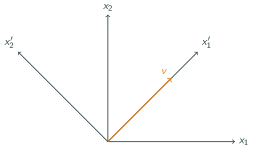
\includegraphics{../images/trans-vector.svg}
\end{frame}

\begin{frame}{coordinate transformation in two dimensions}
\protect\hypertarget{coordinate-transformation-in-two-dimensions-1}{}
\begin{itemize}
\tightlist
\item
  The vector, \emph{v}, remains fixed, but we transform our coordinate
  system
\item
  In the new coordinate system, the \(x_2^\prime\) portion of \emph{v}
  is zero.
\item
  To transform the coordinate system, we first define some unit vectors.
\item
  \(\hat{e}_1\) is a unit vector in the direction of \(x_1\), while
  \(\hat{e}_1^\prime\) is a unit vector in the direction of
  \(x_1^\prime\)
\end{itemize}
\end{frame}

\begin{frame}{coordinate transformation in two dimensions}
\protect\hypertarget{coordinate-transformation-in-two-dimensions-2}{}
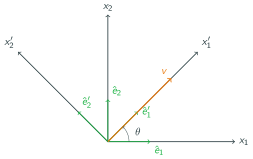
\includegraphics{../images/trans-vec-unit.svg}
\end{frame}

\begin{frame}{coordinate transformation in two dimensions}
\protect\hypertarget{coordinate-transformation-in-two-dimensions-3}{}
\begin{itemize}
\tightlist
\item
  For this example, let us assume \(v = \langle 2, 2 \rangle\) and
  \(\theta = 45^\circ\)
\item
  We can write the transformed unit vectors, \(\hat{e}_1^\prime\) and
  \(\hat{e}_2^\prime\) in terms of \(\hat{e}_1\), \(\hat{e}_2\) and the
  angle of rotation, \(\theta\).
\end{itemize}

\[\begin{aligned}
    \hat{e}_1^\prime &= \langle \hat{e}_1 \cos \theta , \hat{e}_2 \sin \theta \rangle\\
    \hat{e}_2^\prime &= \langle -\hat{e}_1 \sin \theta , \hat{e}_2 \cos \theta \rangle
\end{aligned}\]
\end{frame}

\begin{frame}{coordinate transformation in two dimensions}
\protect\hypertarget{coordinate-transformation-in-two-dimensions-4}{}
\begin{itemize}
\tightlist
\item
  We can write the vector, \emph{v}, in terms of the unit vectors
  describing our axis system
\item
  \(v = v_1 \hat{e}_1 + v_2 \hat{e}_2\)
\item
  (note: \(\hat{e}_1=\langle 1, 0 \rangle\) and
  \(\hat{e}_2 = \langle 0,1 \rangle\))
\item
  \(v = \langle 2, 2 \rangle = 2\langle 1, 0 \rangle + 2\langle 0, 1 \rangle\)
\end{itemize}
\end{frame}

\begin{frame}{coordinate transformation in two dimensions}
\protect\hypertarget{coordinate-transformation-in-two-dimensions-5}{}
\begin{itemize}
\tightlist
\item
  When expressed in the transformed coordinate system, we refer to
  \(v^\prime\)
\item
  \(v^\prime = \langle v_1 \cos \theta + v_2 \sin \theta, -v_1 \sin \theta + v_2 \cos \theta\)
\item
  \(v^\prime = \langle 2\sqrt{2}, 0 \rangle\)
\item
  We can recover the original vector from the transformed coordinates:
\item
  \(v = v_1^\prime \hat{e}_1^\prime + v_2^\prime \hat{e}_2^\prime\)
\item
  (note:
  \(\hat{e}_1^\prime=\langle \frac{\sqrt{2}}{2},\frac{\sqrt{2}}{2} \rangle\)
  and
  \(\hat{e}_2^\prime = \langle -\frac{\sqrt{2}}{2},\frac{\sqrt{2}}{2} \rangle\)\}
\item
  \(v = 2\sqrt{2}\langle \frac{\sqrt{2}}{2},\frac{\sqrt{2}}{2} \rangle, 0 \langle -\frac{\sqrt{2}}{2},\frac{\sqrt{2}}{2} \rangle = \langle 2, 2 \rangle\)
\end{itemize}
\end{frame}

\begin{frame}{general coordinate transformation}
\protect\hypertarget{general-coordinate-transformation}{}
\begin{itemize}
\tightlist
\item
  Coordinate transformation can become much more complicated in three
  dimensions, and with higher-order tensors
\item
  It is convenient to define a general form of the coordinate
  transformation in index notation
\item
  We define \(Q_{ij}\) as the cosine of the angle between the
  \(x_i^\prime\) axis and the \(x_j\) axis.
\item
  This is also referred to as the ``direction cosine''
\end{itemize}

\[Q_{ij} = \cos(x_i^\prime, x_j)\]
\end{frame}

\begin{frame}{mental and emotional health warning}
\protect\hypertarget{mental-and-emotional-health-warning}{}
\begin{itemize}
\tightlist
\item
  Different textbooks flip the definition of \(Q_{ij}\) (Elasticity and
  Continuum texts have opposite definitions, for example)
\item
  The result gives the transpose
\item
  Always use equations (next slide) from the same source as your
  \(Q_{ij}\) definition
\end{itemize}
\end{frame}

\begin{frame}{general coordinate transformation}
\protect\hypertarget{general-coordinate-transformation-1}{}
\begin{itemize}
\tightlist
\item
  We can transform any-order tensor using \(Q_{ij}\)
\item
  Vectors (first-order tensors): \(v_i^\prime = Q_{ij} v_j\)
\item
  Matrices (second-order tensors):
  \(\sigma_{ij}^\prime = Q_{im}Q_{jn} \sigma_{mn}\)
\item
  Fourth-order tensors:
  \(C_{ijkl}^\prime = Q_{im}Q_{jn}Q_{ko}Q_{lp} C_{mnop}\)
\end{itemize}
\end{frame}

\begin{frame}{general coordinate transformation}
\protect\hypertarget{general-coordinate-transformation-2}{}
\begin{itemize}
\tightlist
\item
  We can use this form on our 2D transformation example
\end{itemize}

\[\begin{aligned}
  Q_{ij} &= \cos (x_i^\prime, x_j)\ &=
  \begin{bmatrix}
  \cos (x_1^\prime, x_1) & \cos (x_1^\prime, x_2)\\
  \cos (x_2^\prime, x_1) & \cos (x_2^\prime, x_2)
  \end{bmatrix}\\
  &= \begin{bmatrix}
  \cos \theta & \cos (90-\theta)\\
  \cos (90+\theta) & \cos \theta
  \end{bmatrix} \\
  &= \begin{bmatrix}
  \cos \theta & \sin \theta \\
  -\sin \theta & \cos \theta
  \end{bmatrix}
\end{aligned}\]
\end{frame}

\begin{frame}{general coordinate transformation}
\protect\hypertarget{general-coordinate-transformation-3}{}
\begin{itemize}
\tightlist
\item
  We can similarly use \(Q_{ij}\) to find tensors in the original
  coordinate system
\item
  Vectors (first-order tensors): \(v_j = Q_{ij} v_i^\prime\)
\item
  Matrices (second-order tensors):
  \(\sigma_{mn} = Q_{im}Q_{jn} \sigma_{ij}^\prime\)
\item
  Fourth-order tensors:
  \(C_{mnop} = Q_{im}Q_{jn}Q_{ko}Q_{lp} C_{ijkl}^\prime\)
\end{itemize}
\end{frame}

\begin{frame}{general coordinate transformation}
\protect\hypertarget{general-coordinate-transformation-4}{}
\begin{itemize}
\tightlist
\item
  We can derive some interesting properties of the transformation
  tensor, \(Q_{ij}\)
\item
  We know that \(v_i^\prime = Q_{ij} v_j\) and that
  \(v_j = Q_{ij} v_i^\prime\)
\item
  If we substitute (changing the appropriate indexes) we find:
\item
  \(v_j = Q_{ij} Q_{ik} v_k\)
\item
  We can now use the Kronecker Delta to substitute
  \(v_j = \delta_{jk}v_k\)
\item
  \(\delta_{jk}v_k = Q_{ij} Q_{ik} v_k\)
\end{itemize}
\end{frame}

\hypertarget{examples}{%
\section{examples}\label{examples}}

\begin{frame}{example}
\protect\hypertarget{example}{}
\begin{columns}[T]
\begin{column}{0.5\textwidth}
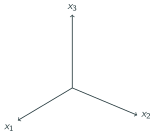
\includegraphics{../images/3d-axis.svg}
\end{column}

\begin{column}{0.5\textwidth}
\begin{itemize}
\tightlist
\item
  Find \(Q_{ij}^1\) for rotation of \(60^\circ\) about \(x_2\)
\item
  Find \(Q_{ij}^2\) for rotation of \(30^\circ\) about \(x_3^\prime\)
\item
  Find \(e_{i}^{\prime\prime}\) after both rotations
\end{itemize}
\end{column}
\end{columns}
\end{frame}

\begin{frame}{example}
\protect\hypertarget{example-1}{}
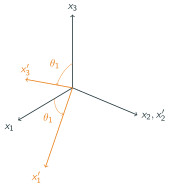
\includegraphics{../images/3d-y-rot.svg}
\end{frame}

\begin{frame}{example}
\protect\hypertarget{example-2}{}
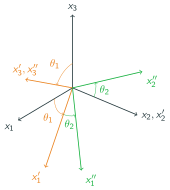
\includegraphics{../images/3d-z-rot.svg}
\end{frame}

\begin{frame}{example}
\protect\hypertarget{example-3}{}
\begin{itemize}
\tightlist
\item
  \(Q_{ij}^1 = \cos(x_i^\prime,x_j)\)
\item
  \(Q_{ij}^2 = \cos(x_i^{\prime\prime},x_j^\prime)\)
\end{itemize}

\[Q_{ij}^1 = \begin{bmatrix}
  \cos 60 & \cos 90 & \cos 150\\
  \cos 90 & \cos 0 & \cos 90\\
  \cos 30 & \cos 90 & \cos 60
\end{bmatrix}\]

\[Q_{ij}^2 = \begin{bmatrix}
  \cos 30 & \cos 60 & \cos 90\\
  \cos 120 & \cos 30 & \cos 90\\
  \cos 90 & \cos 90 & \cos 0
\end{bmatrix}\]
\end{frame}

\begin{frame}{example}
\protect\hypertarget{example-4}{}
\begin{itemize}
\tightlist
\item
  We now use \(Q_{ij}\) to find \(\hat{e}_i^\prime\) and
  \(\hat{e}_i^{\prime \prime}\)
\item
  First, we need to write \(\hat{e}_i\) in a manner more consistent with
  index notation
\item
  We will indicate axis direction with a superscript,
  e.g.~\(\hat{e}_1 = e_i^1\)
\item
  \(e_i^\prime = Q_{ij}^1 e_j\)
\item
  \(e_i^{\prime\prime} = Q_{ij}^2 e_j^\prime\)
\item
  How do we find \(e_i^{\prime\prime}\) in terms of \(e_i\)?
\end{itemize}
\end{frame}

\hypertarget{anisotropic-elasticity}{%
\section{anisotropic elasticity}\label{anisotropic-elasticity}}

\begin{frame}{stiffness}
\protect\hypertarget{stiffness}{}
\begin{itemize}
\tightlist
\item
  In 3D, Hooke's Law for linearly elastic materials is
\end{itemize}

\[\sigma_{ij} = C_{ijkl} \epsilon_{kl}\]

\begin{itemize}
\tightlist
\item
  For isotropic materials, \(C_{ijkl}\) can be expressed in terms of two
  constants
\item
  In general (anisotropic materials) more constants are needed and we
  use the full tensor
\end{itemize}
\end{frame}

\begin{frame}{engineering notation}
\protect\hypertarget{engineering-notation}{}
\begin{itemize}
\tightlist
\item
  Fourth-order tensors are cumbersome to write, we often use engineering
  notation
\item
  \(\sigma\) and \(\epsilon\) are written as vectors and \(C_{ijkl}\) is
  written as a matrix.
\item
  NOTE: Although \(\sigma\), \(\epsilon\) and \(C_{ijkl}\) are tensors,
  their counterparts in engineering notation are NOT formal tensors
\item
  This means that the usual transformation laws do not apply
\end{itemize}
\end{frame}

\begin{frame}{engineering notation}
\protect\hypertarget{engineering-notation-1}{}
\[\begin{bmatrix}
  \sigma_{11}\ \sigma_{22} \ \sigma_{33} \ \sigma_{23} \ \sigma_{13} \ \sigma_{12}
  \end{bmatrix}
  = \begin{bmatrix}
  C_{1111} & C_{1122} & C_{1133} & C_{1123} & C_{1113} & C_{1112} \\
  C_{1122} & C_{2222} & C_{2233} & C_{2223} & C_{1322} & C_{1222} \\
  C_{1133} & C_{2233} & C_{3333} & C_{2333} & C_{1333} & C_{1233} \\
  C_{1123} & C_{2223} & C_{2333} & C_{2323} & C_{1323} & C_{1223} \\
  C_{1113} & C_{1322} & C_{1333} & C_{1323} & C_{1313} & C_{1213} \\
  C_{1112} & C_{1222} & C_{1233} & C_{1223} & C_{1213} & C_{1212}
  \end{bmatrix}\begin{bmatrix}
  E_{11} \ E_{22} \ E_{33} \2E_{23} \ 2E_{13} \ 2E_{12}
\end{bmatrix}\]
\end{frame}

\begin{frame}{compliance}
\protect\hypertarget{compliance}{}
\[\begin{bmatrix}
  E_{11} \ E_{22} \ E_{33} \2E_{23} \ 2E_{13} \ 2E_{12}
  \end{bmatrix}
  = \begin{bmatrix}
  S_{1111} & S_{1122} & S_{1133} & S_{1123} & S_{1113} & S_{1112} \\
  S_{1122} & S_{2222} & S_{2233} & S_{2223} & S_{1322} & S_{1222} \\
  S_{1133} & S_{2233} & S_{3333} & S_{2333} & S_{1333} & S_{1233} \\
  S_{1123} & S_{2223} & S_{2333} & S_{2323} & S_{1323} & S_{1223} \\
  S_{1113} & S_{1322} & S_{1333} & S_{1323} & S_{1313} & S_{1213} \\
  S_{1112} & S_{1222} & S_{1233} & S_{1223} & S_{1213} & S_{1212}
  \end{bmatrix}\begin{bmatrix}
  \sigma_{11} \ \sigma_{22} \ \sigma_{33} \ \sigma_{23} \ \sigma_{13} \ \sigma_{12}
\end{bmatrix}\]
\end{frame}

\begin{frame}{physical interpretation}
\protect\hypertarget{physical-interpretation}{}
\begin{itemize}
\tightlist
\item
  If we now consider the case of uniaxial tension, we see that
\end{itemize}

\[\begin{aligned}
  E_{11} &= S_{1111} \sigma_{11}\\
  E_{22} &= S_{1122} \sigma_{11}\\
  E_{33} &= S_{1133} \sigma_{11}\\
  2E_{23} &= S_{1123} \sigma_{11}\\
  2E_{13} &= S_{1113} \sigma_{11}\\
  2E_{12} &= S_{1112} \sigma_{11}
\end{aligned}\]

\begin{itemize}
\tightlist
\item
  \emph{S}1111 is familiar, acting like 1/\emph{E}\emph{Y}
\end{itemize}
\end{frame}

\begin{frame}{poisson's ratio}
\protect\hypertarget{poissons-ratio}{}
\begin{itemize}
\tightlist
\item
  For isotropic materials we defined Poisson's ratio as
  \(\nu = -E_{22}/E_{11}\)
\item
  For anisotropic materials, we can have a different Poisson's ratio
  acting in different directions
\item
  We define \(\nu_{ij} = -E_{jj}/E_{ii}\) (with no summation), the ratio
  of the transverse strain in the \emph{j} direction when stress is
  applied in the \emph{i} direction
\item
  For this example we can find \(\nu_{12}\) and \(\nu_{13}\) as
\end{itemize}

\[\begin{aligned}
  \nu_{12} &= -E_{22}/E_{11} = -S_{1122}/S_{1111}\\
  \nu_{13} &= -E_{33}/E_{11} = -S_{1133}/S_{1111}
\end{aligned}\]
\end{frame}

\begin{frame}{poisson's ratio}
\protect\hypertarget{poissons-ratio-1}{}
\begin{itemize}
\tightlist
\item
  Note that we cannot, in general, say that \(\nu_{12} = \nu_{21}\)
\item
  However, due to the symmetry of the stiffness/compliance tensors, we
  know that
\end{itemize}

\[\begin{aligned}
  \nu_{21} E_{x} &= \nu_{12} E_{y}\\
  \nu_{31} E_{x} &= \nu_{13} E_{z}\\
  \nu_{32} E_{y} &= \nu_{23} E_{z}
\end{aligned}\]

\begin{itemize}
\tightlist
\item
  Where \(E_x\) refer's to the Young's Modulus in the
  \emph{x}-direction, etc.
\end{itemize}
\end{frame}

\begin{frame}{shear coupling coefficients}
\protect\hypertarget{shear-coupling-coefficients}{}
\begin{itemize}
\tightlist
\item
  An unfamiliar effect is that shear strains can be introduced from a
  normal stress
\item
  We define shear coupling coefficients as
  \(\eta_{1112} = \eta_{16} = -2E_{12}/E_{11}\) due to \(\sigma_{11}\)
\item
  These coupling terms can also effect shear strain in a different plane
  from the applied shear stress
\item
  Like the Poisson's ratio, these are not entirely independent
\end{itemize}

\[ \eta_{61} E_x = \eta_{16} G_6 \]

\begin{itemize}
\tightlist
\item
  Where \(G_6\) is the shear modulus in the 12 plane
\end{itemize}
\end{frame}

\begin{frame}{shear coupling coefficients}
\protect\hypertarget{shear-coupling-coefficients-1}{}
\begin{itemize}
\tightlist
\item
  Shear coupling coefficients are sometimes placed in two groups
\item
  Coefficients of mutual influence relate shear stress to normal strain
  and normal stress to shear strain
\item
  Chentsov coefficients relate shear stress in one plane to shear strain
  in another plane
\item
  In general we can say
\end{itemize}

\[\eta_{nm} E_m = \eta_{mn} G_n \qquad \text{(m = 1,2,3) (n = 4,5,6)} \]

and

\[\eta_{nm} G_m = \eta_{mn} G_n \qquad \text{(m,n = 4,5,6)} \qquad m \ne n \]
\end{frame}

\begin{frame}{orthotropic symmetry}
\protect\hypertarget{orthotropic-symmetry}{}
\[\small \begin{bmatrix}
  \sigma_{11}\ \sigma_{22} \ \sigma_{33} \\sigma_{23} \ \sigma_{13} \ \sigma_{12}
  \end{bmatrix}
  = \begin{bmatrix}
  C_{1111} & C_{1122} & C_{1133} & 0 & 0 & 0 \\
  C_{1122} & C_{2222} & C_{2233} & 0 & 0 & 0 \\
  C_{1133} & C_{2233} & C_{3333} & 0 & 0 & 0 \\
  0 & 0 & 0 & C_{2323} & 0 & 0 \\
  0 & 0 & 0 & 0 & C_{1313} & 0 \\
  0 & 0 & 0 & 0 & 0 & C_{1212}
  \end{bmatrix}\begin{bmatrix}
  E_{11}\ E_{22} \ E_{33} \2E_{23} \ 2E_{13} \ 2E_{12}
\end{bmatrix}\]
\end{frame}

\begin{frame}{transversely isotropic symmetry}
\protect\hypertarget{transversely-isotropic-symmetry}{}
\[\small \begin{bmatrix}
  \sigma_{11}\ \sigma_{22} \ \sigma_{33} \\sigma_{23} \ \sigma_{13} \ \sigma_{12}
  \end{bmatrix}
  = \begin{bmatrix}
  C_{1111} & C_{1122} & C_{1133} & 0 & 0 & 0 \\
  C_{1122} & C_{1111} & C_{1133} & 0 & 0 & 0 \\
  C_{1133} & C_{1133} & C_{3333} & 0 & 0 & 0 \\
  0 & 0 & 0 & C_{1313} & 0 & 0 \\
  0 & 0 & 0 & 0 & C_{1313} & 0 \\
  0 & 0 & 0 & 0 & 0 & 1/2(C_{1111}-C_{2222})
  \end{bmatrix}\begin{bmatrix}
  E_{11}\ E_{22} \ E_{33} \2E_{23} \ 2E_{13} \ 2E_{12}
\end{bmatrix}\]
\end{frame}

\begin{frame}{isotropic symmetry}
\protect\hypertarget{isotropic-symmetry}{}
\[\scriptsize \begin{bmatrix}
  \sigma_{11}\ \sigma_{22} \ \sigma_{33} \\sigma_{23} \ \sigma_{13} \ \sigma_{12}
  \end{bmatrix}
  = \frac{E}{(1+\nu)(1-2\nu)}\begin{bmatrix}
  1-\nu & \nu & \nu & 0 & 0 & 0 \\
  \nu & 1-\nu & \nu & 0 & 0 & 0 \\
  \nu & \nu & 1-\nu & 0 & 0 & 0 \\
  0 & 0 & 0 & \frac{1}{2}(1-2\nu) & 0 & 0 \\
  0 & 0 & 0 & 0 & \frac{1}{2}(1-2\nu) & 0 \\
  0 & 0 & 0 & 0 & 0 & \frac{1}{2}(1-2\nu)
  \end{bmatrix}\begin{bmatrix}
  E_{11}\ E_{22} \ E_{33} \2E_{23} \ 2E_{13} \ 2E_{12}
\end{bmatrix}\]
\end{frame}

\begin{frame}{next class}
\protect\hypertarget{next-class}{}
\begin{itemize}
\tightlist
\item
  Next class we will develop transformation laws for engineering
  stress/strain and stiffness
\end{itemize}
\end{frame}

\end{document}
